%!TEX root = ../final.tex
% This question is basically ripped off from fa16 midterm
\question This question uses the following histogram of the number of gallons
of fuel consumed by different ships on the same trip.

\begin{figure}[h!]
  \centering
  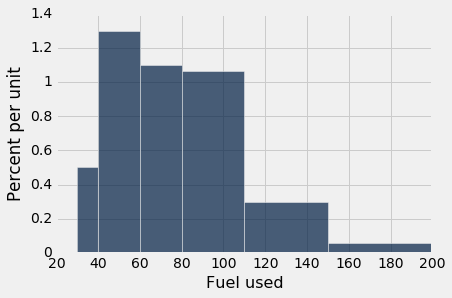
\includegraphics[height=5cm]{figs/fuel_bins.png}
  \label{fig:fuelbins}
\end{figure}

The heights of the bars (in percent per gallon of fuel) are:

\begin{center}
\begin{tabular}{ r || c | c | c | c | c | c }
 bin & [30, 40) & [40, 60) & [60, 80)
    & [80, 110) & [110, 150) & [150, 200) \\
 \hline
 height & 0.5 & 1.3 & 1.1 & 1.07 & ? & 0.06 \\
\end{tabular}
\end{center}

\begin{parts}
  \part[3] Find the missing bin height in percent per gallon of fuel. You may
  leave your answer as an expression. If it is not possible to find the height,
  explain why.

  \begin{solutionorbox}[1in]
  The areas of the bars must sum to 100 percent, so:
  \begin{align*}
    \frac{100 - 10(0.5) - 20(1.3) - 20(1.1) - 30(1.07) - 50(0.06)}{40} \approx
    0.296
  \end{align*}
  \end{solutionorbox}

  \part[3] Without any extra information, which bin has the most ships?

  \begin{oneparcheckboxes}
    \choice [40, 60)
    \choice [60, 80)
    \choice [80, 110)
    \choice Can't determine without additional information.
  \end{oneparcheckboxes}

  Justify your choice. If you picked the last choice, state the extra
  information you need.

  \begin{solutionorbox}[.7in]
  The [40, 60) bar has an area of: $ 20 * 1.3 = 26\% $.
  The [60, 80) bar has an area of: $ 20 * 1.1 = 22\% $.
  The [80, 110) bar has an area of: $ 30 * 1.07 = 30.21\% $.

  So, the [80, 110) bin has more ships regardless of how many ships there are total.
  \end{solutionorbox}

  \part[4] Suppose we merge the [30, 40) and [40, 60) bin together to create a
  single bin for [30, 60). What is the new height of [30, 60) bin (in percent
  per gallon)? You may leave your answer as an expression. If you need more
  information, state the information you need.

  \begin{solutionorbox}[2in]
  The [30, 40) bin has an area of: $ 10(0.5) = 5\% $. The [40, 60) bin has an area
  of $ 20(1.3) = 26\% $.

  The total area is then $ 31\% $. Dividing by the total width of the new bin
  we have a height of: $ 31 / (30) \approx 1.03 $.

  Note that you didn't need to know the number of ships in the [30, 40) bin to
  solve this problem!
  \end{solutionorbox}
\end{parts}
